\section{Az adatgyűjtés folyamata}

A mélytanulási modellek betanításának alapfeltétele egy kellő méretű, változatos és reprezentatív
annotált képadathalmaz. Jelen projekt esetén ez különösen nehéz feladatnak bizonyult: az FDM
nyomtatási hibák vizuális megjelenése rendkívül változatos, függ a nyomtató típusától, a filament
anyagától és színétől, a megvilágítástól, a kamera szögétől és felbontásától, valamint a hiba
súlyosságától. Egy ilyen feltételek mellett általánosítható modell betanításához tehát nagy forrásvariabilitással rendelkező adathalmazra van szükség.

Az adatgyűjtés több párhuzamos forrásra támaszkodott: nyilvánosan elérhető adathalmazokra,
automatizált webes képletöltésre, valamint saját kezűleg rögzített felvételekre.

    \subsection{Nyilvánosan elérhető adathalmazok}

    Az adatgyűjtés első lépéseként három publikusan elérhető, 3D nyomtatási hibákat tartalmazó
    adathalmaz került felhasználásra.

    A Kaggle platformon Padraig Valenti által közzétett \textit{3D Printing Failure Detection}
    adathalmaz~\cite{kaggle_valenti} már YOLO-kompatibilis formátumban tartalmaz annotált képeket
    a legelterjedtebb FDM-hibatípusokra.

    A szintén Kaggle-ön elérhető, \textit{Mikulhe} felhasználó által megosztott \textit{3D Printing
    Errors}~\cite{kaggle_mikulhe} adathalmaz kiegészítő felvételeket biztosított, amelyek részben
    eltérő nyomtatókörnyezetből és megvilágítási feltételek mellől származnak, így növelve az
    adathalmaz vizuális diverzitását.

    A HuggingFace platformon a \textit{Javiai/failures-3D-print}~\cite{hf_javiai} adathalmaz
    további, különböző forrásból összegyűjtött hibás nyomtatásokat tartalmazó képeket nyújtott.

    \subsection{Webes képgyűjtés}

    A meglévő adathalmazok kiegészítéseképpen egyedi Python-szkript segítségével automatizált
    webes képletöltés is zajlott. A \texttt{imagescraper.py} szkript két üzemmódban képes működni:
    URL-listából történő közvetlen letöltés, illetve adott weboldal \texttt{<img>} tagjainak
    automatikus kinyerésével végzett oldalfeltérképezés (\textit{web crawling}).
    A letöltés aszinkron módon, az \texttt{aiohttp} könyvtár segítségével valósul meg, párhuzamos
    kapcsolatokkal, újrapróbálkozással és atomi fájlírással, megakadályozva a sérült vagy
    részleges letöltések bekerülését az adathalmazba. Az így összegyűjtött képek manuális
    szűrést követően kerültek az adathalmazba.

    \subsection{Saját felvételek}

    A külső forrásokból gyűjtött képanyagot 397 saját készítésű felvétellel egészítettük ki.
    Ezek valódi nyomtatási folyamatok közben, illetve szándékosan előidézett hibák dokumentálásával
    keletkeztek, a projekt által használt hardverkörnyezetben, azonos kameraelrendezéssel és
    megvilágítási feltételekkel. A saját képek bevonása azért bizonyult fontosnak, mert az
    adathalmaz így tartalmaz a rendszer tényleges működési körülményeihez közel álló felvételeket,
    amelyek segítenek csökkenteni a domain-eltolódás (\textit{domain shift}) hatását.

    Az összes forrásból összegyűjtött, manuálisan szűrt és előkészített adathalmaz az annotálás
    előtt összesen \textbf{2422 képből} állt.

% -------------------------------------------------------------------
\section{Annotálás}

    Az összegyűjtött képek annotálása a CVAT (\textit{Computer Vision Annotation Tool})~\cite{cvat}
    nyílt forráskódú platformon történt, kézi módszerrel. Minden képen az összes látható hibaterület
    körül határoló dobozt (\textit{bounding box}) rajzoltunk, amelyet a megfelelő osztálycímkével
    láttunk el.

    Az annotálás során alkalmazott kilenc osztály a következő:

    \begin{itemize}
        \item \textbf{stringing} - szálazás
        \item \textbf{warping} - vetemedés
        \item \textbf{layer\_shift} - réteg-eltolódás
        \item \textbf{under\_extrusion} - alul-extrúdálás
        \item \textbf{over\_extrusion} - felül-extrúdálás
        \item \textbf{nozzle\_clog} - fúvóka-dugulás
        \item \textbf{foreign\_object\_on\_print\_area} - idegen tárgy a tárgyasztalon
        \item \textbf{not\_sticking} - nem tapadó első réteg
        \item \textbf{spagetti} - spagetti-jelenség
    \end{itemize}

    A \ref{fig:training_grid}. ábra az egyes hibaosztályokhoz tartozó egy-egy reprezentatív tanítóképet mutat be.

    \begin{figure}[H]
    \centering
        \subfigure[szálazás]{
            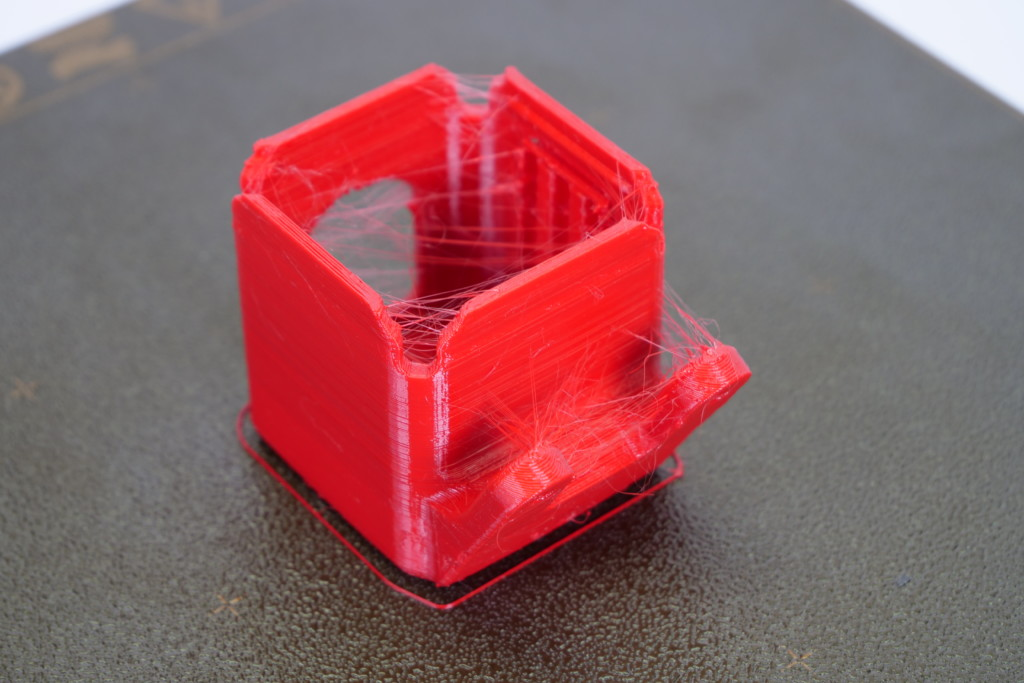
\includegraphics[width=0.3\textwidth]{figures/images/training_samples/stringing.jpg}
        }
        \subfigure[vetemedés]{
            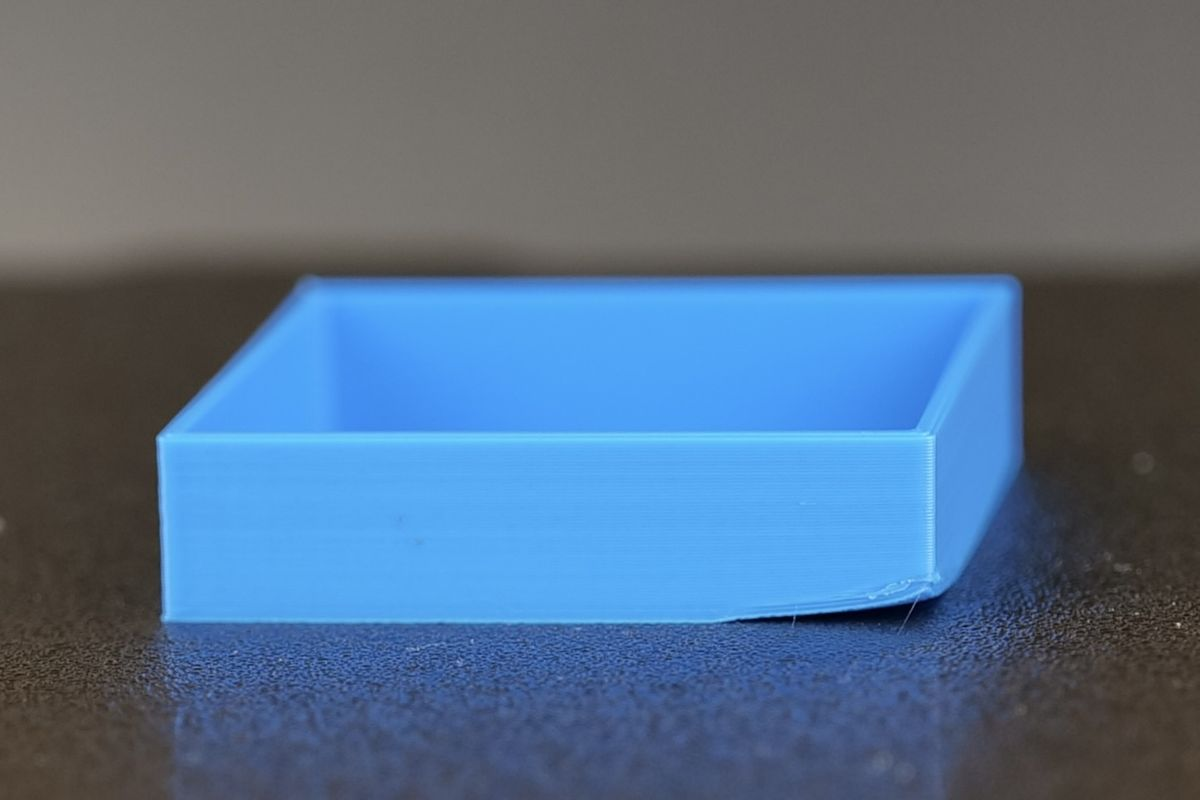
\includegraphics[width=0.3\textwidth]{figures/images/training_samples/warping.jpg}
        }
        \subfigure[réteg eltolódás]{
            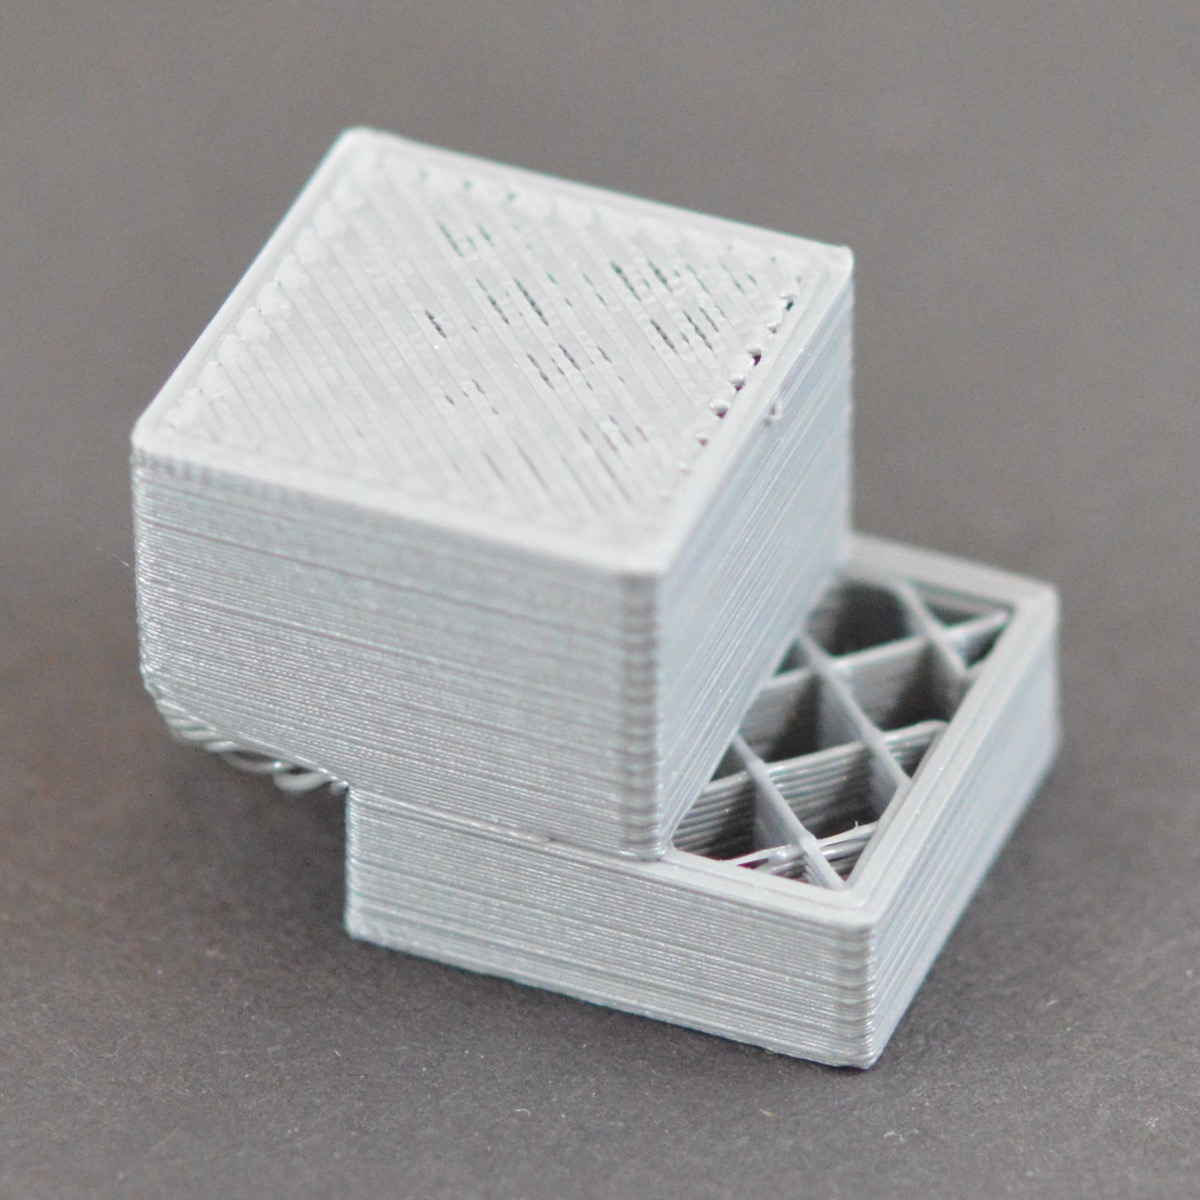
\includegraphics[width=0.3\textwidth]{figures/images/training_samples/layer_shift.jpg}
        }

        \subfigure[alul extrúdálás]{
            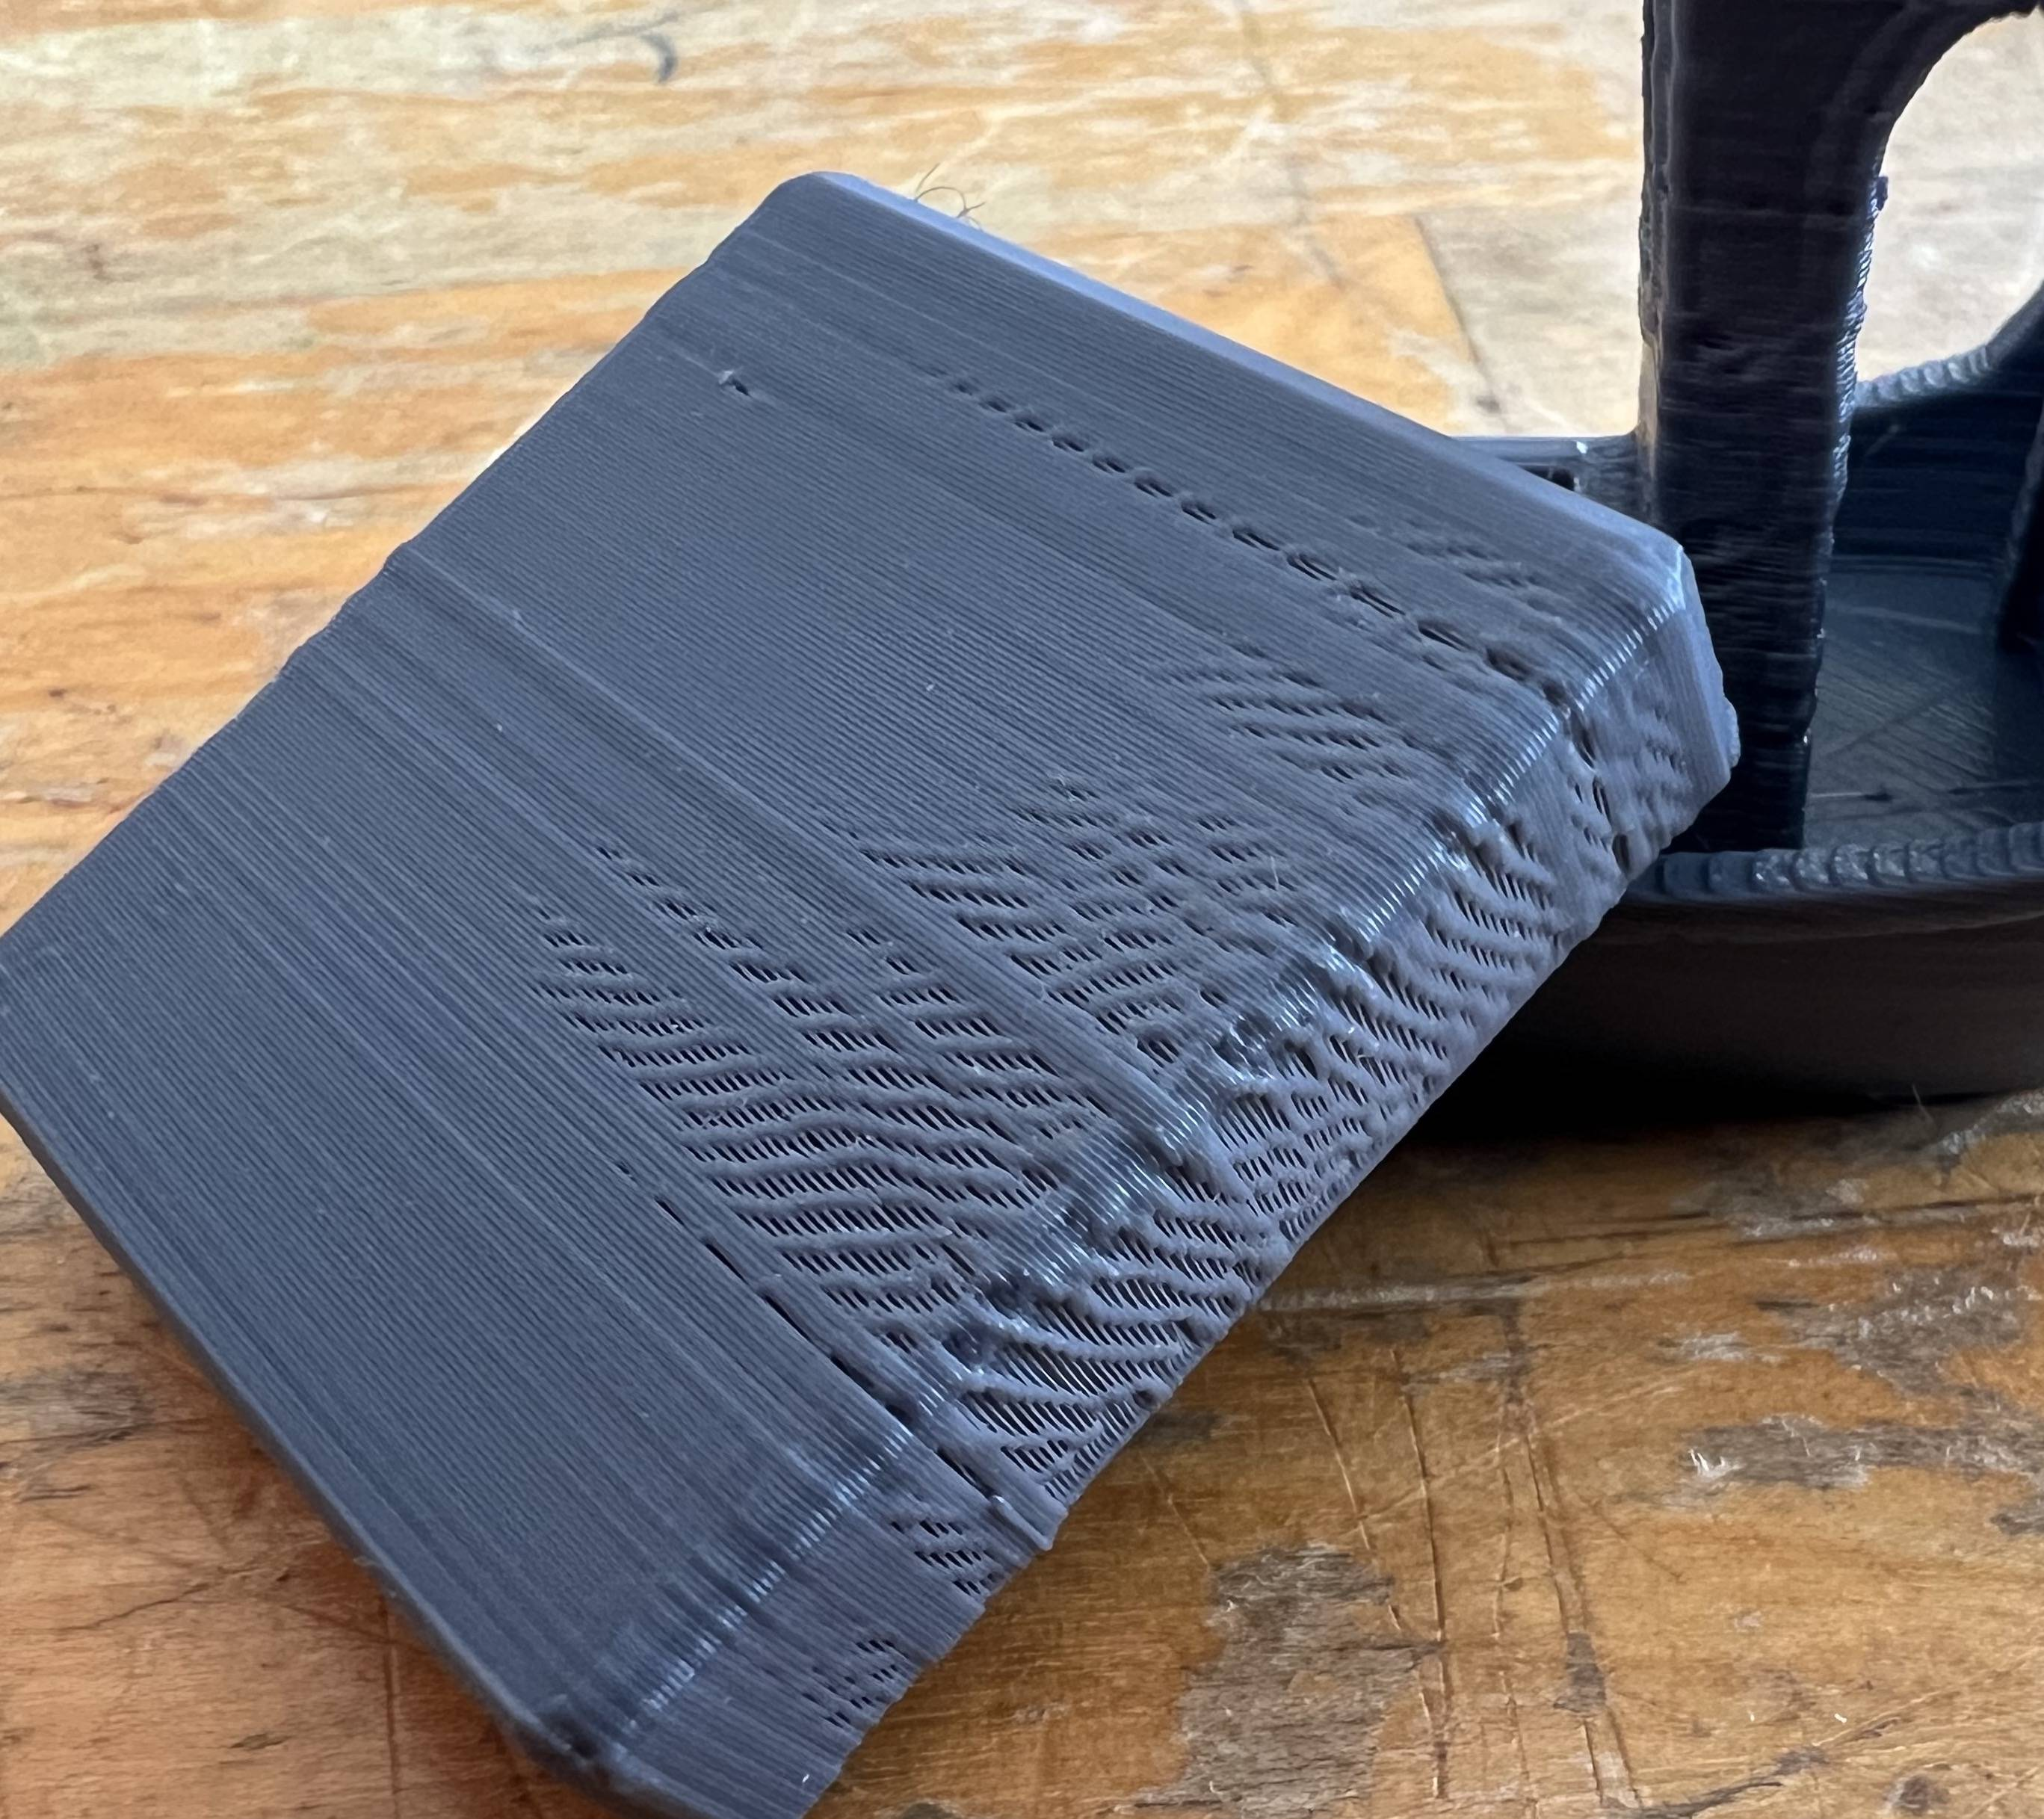
\includegraphics[width=0.3\textwidth]{figures/images/training_samples/under_extrusion.jpg}
        }
        \subfigure[felül extrudálás]{
            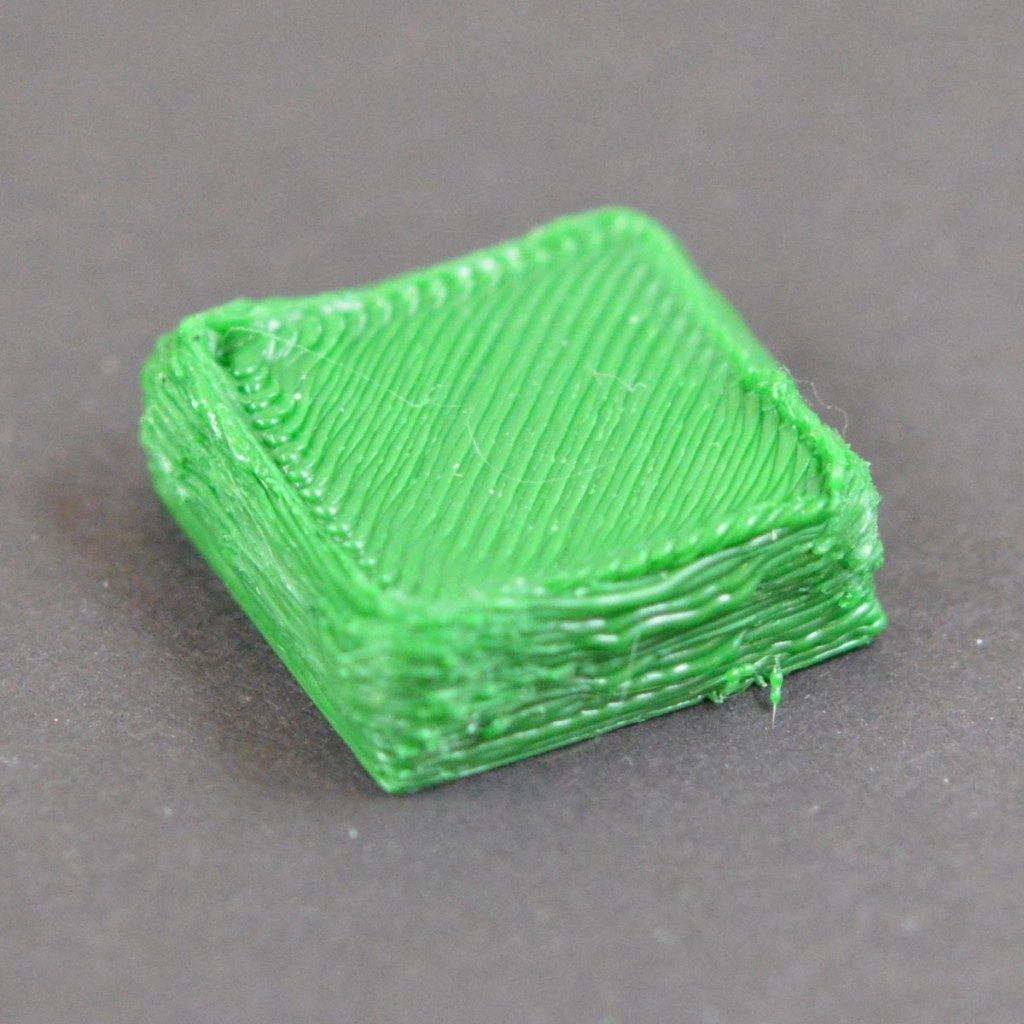
\includegraphics[width=0.3\textwidth]{figures/images/training_samples/over_extrusion.jpg}
        }
        \subfigure[fúvóka dugulás]{
            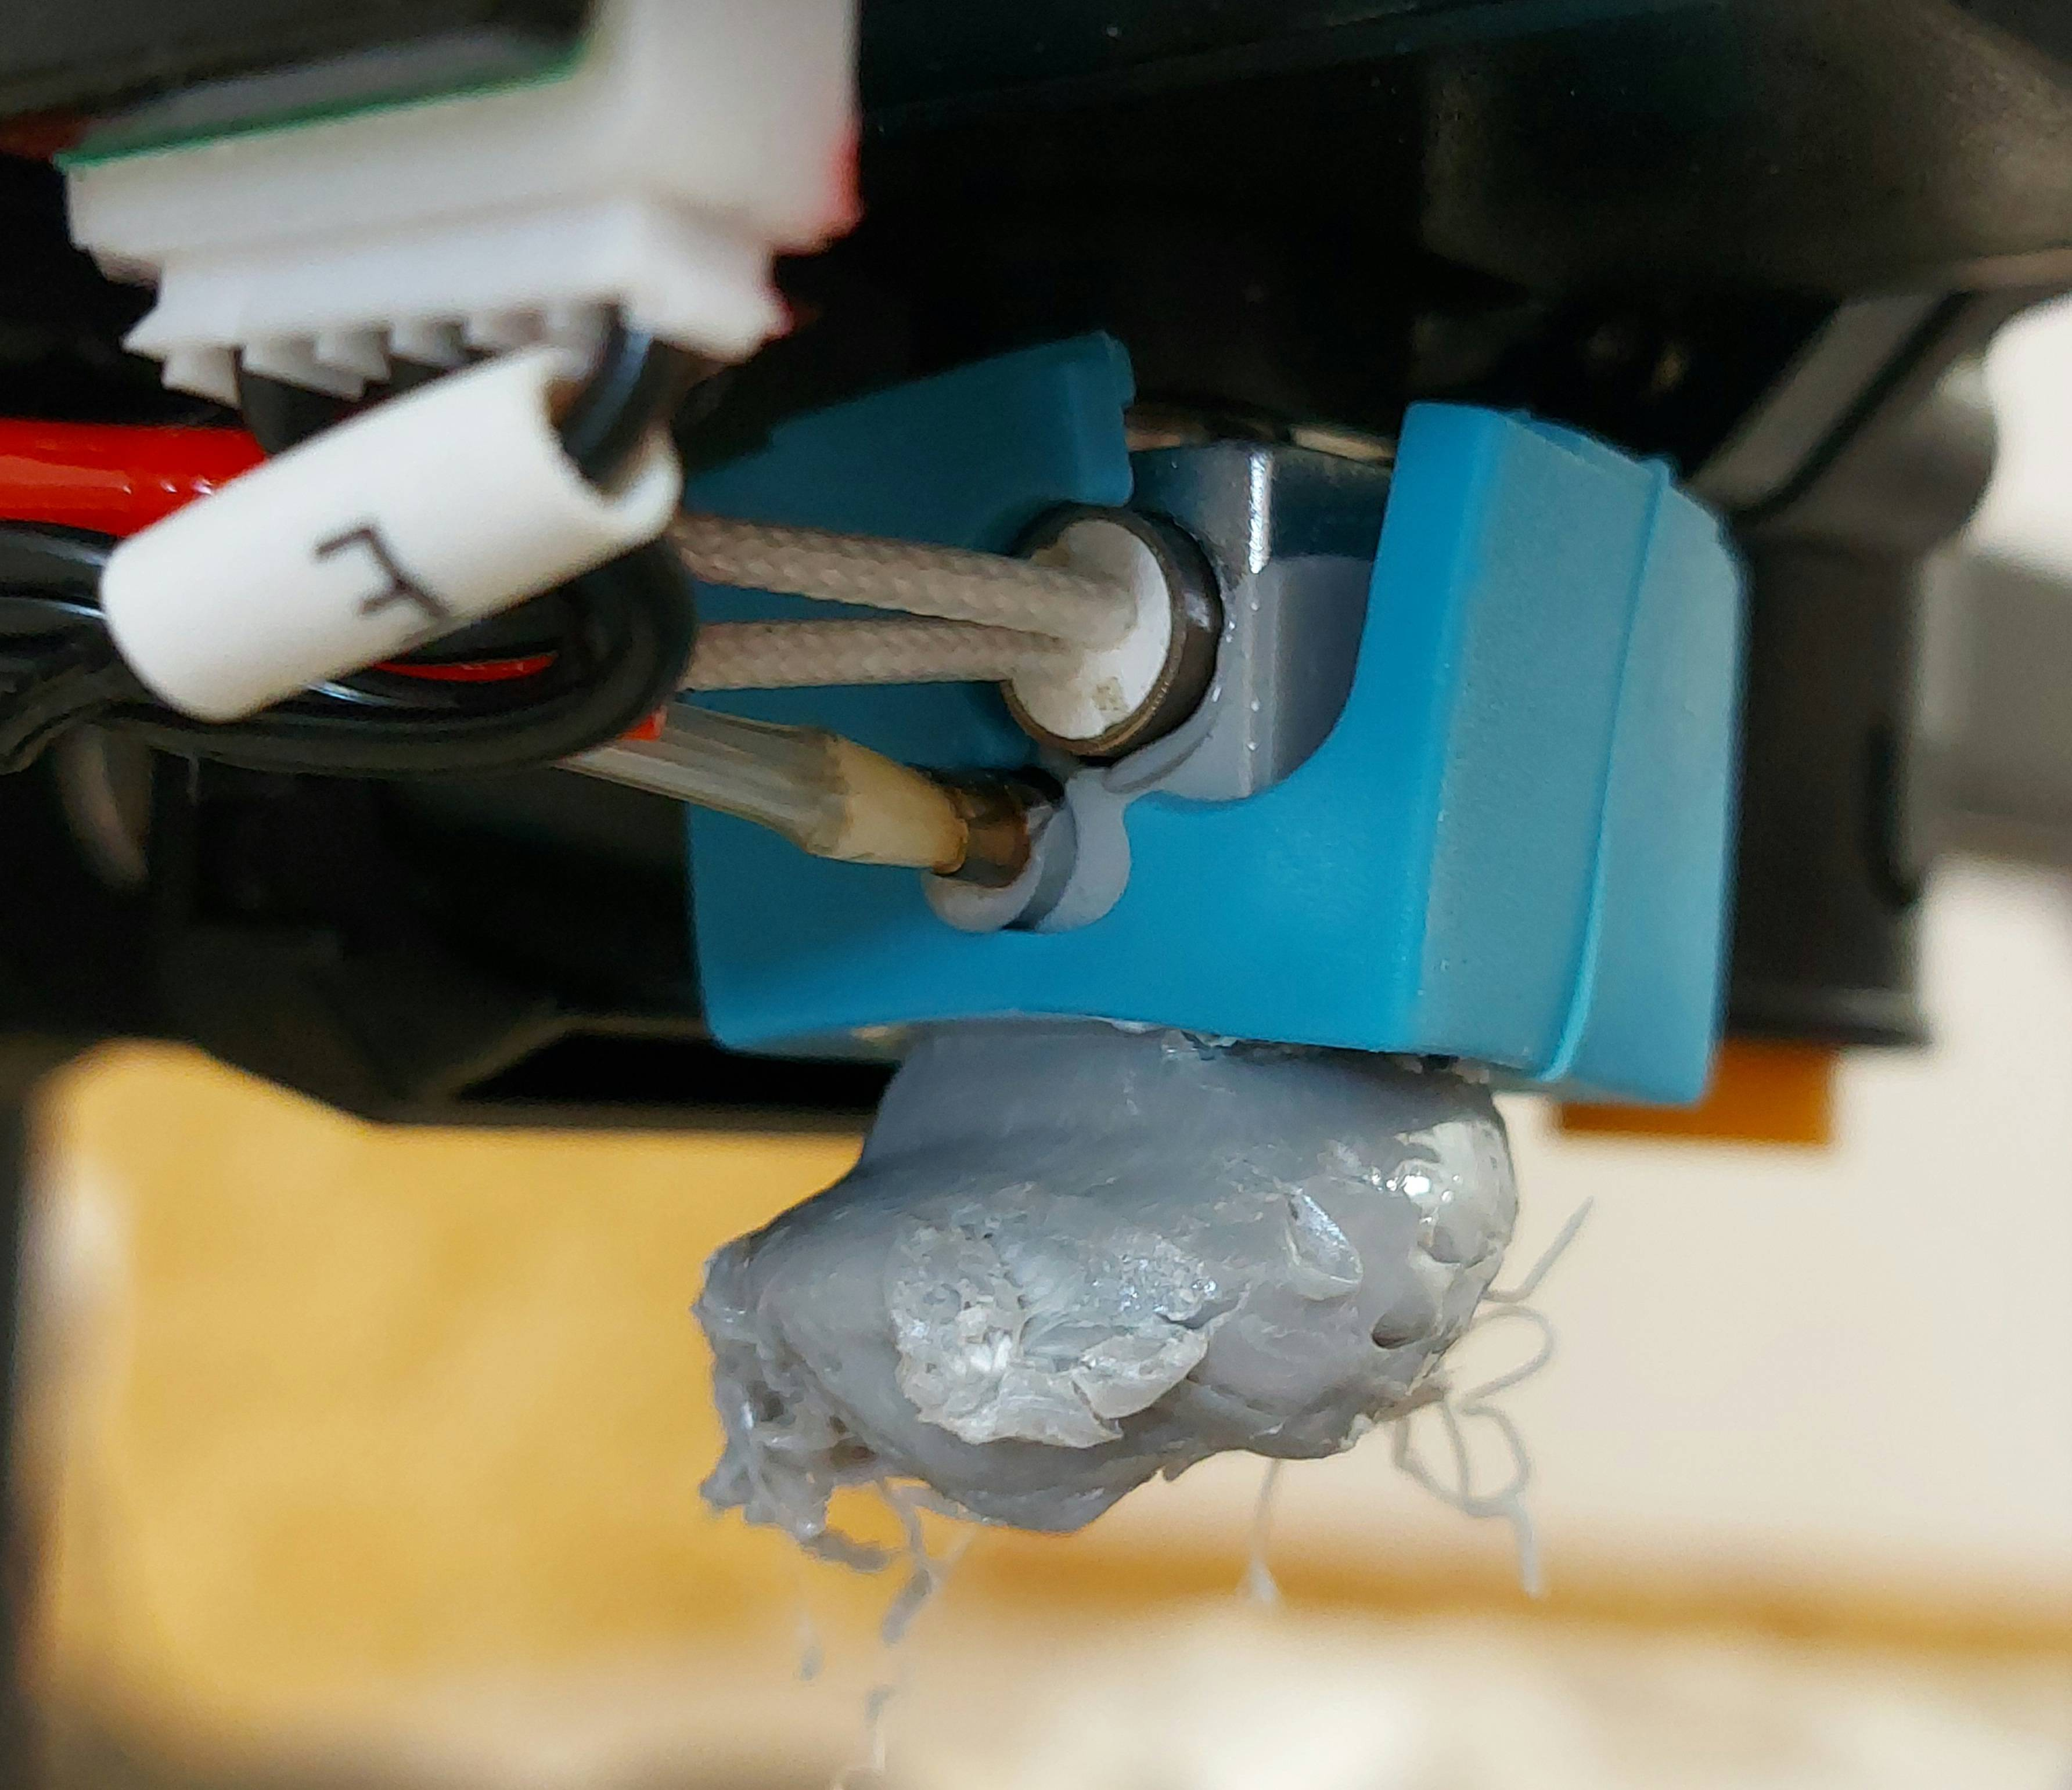
\includegraphics[width=0.3\textwidth]{figures/images/training_samples/nozzle_clog.jpg}
        }

        \subfigure[idegen tárgy]{
            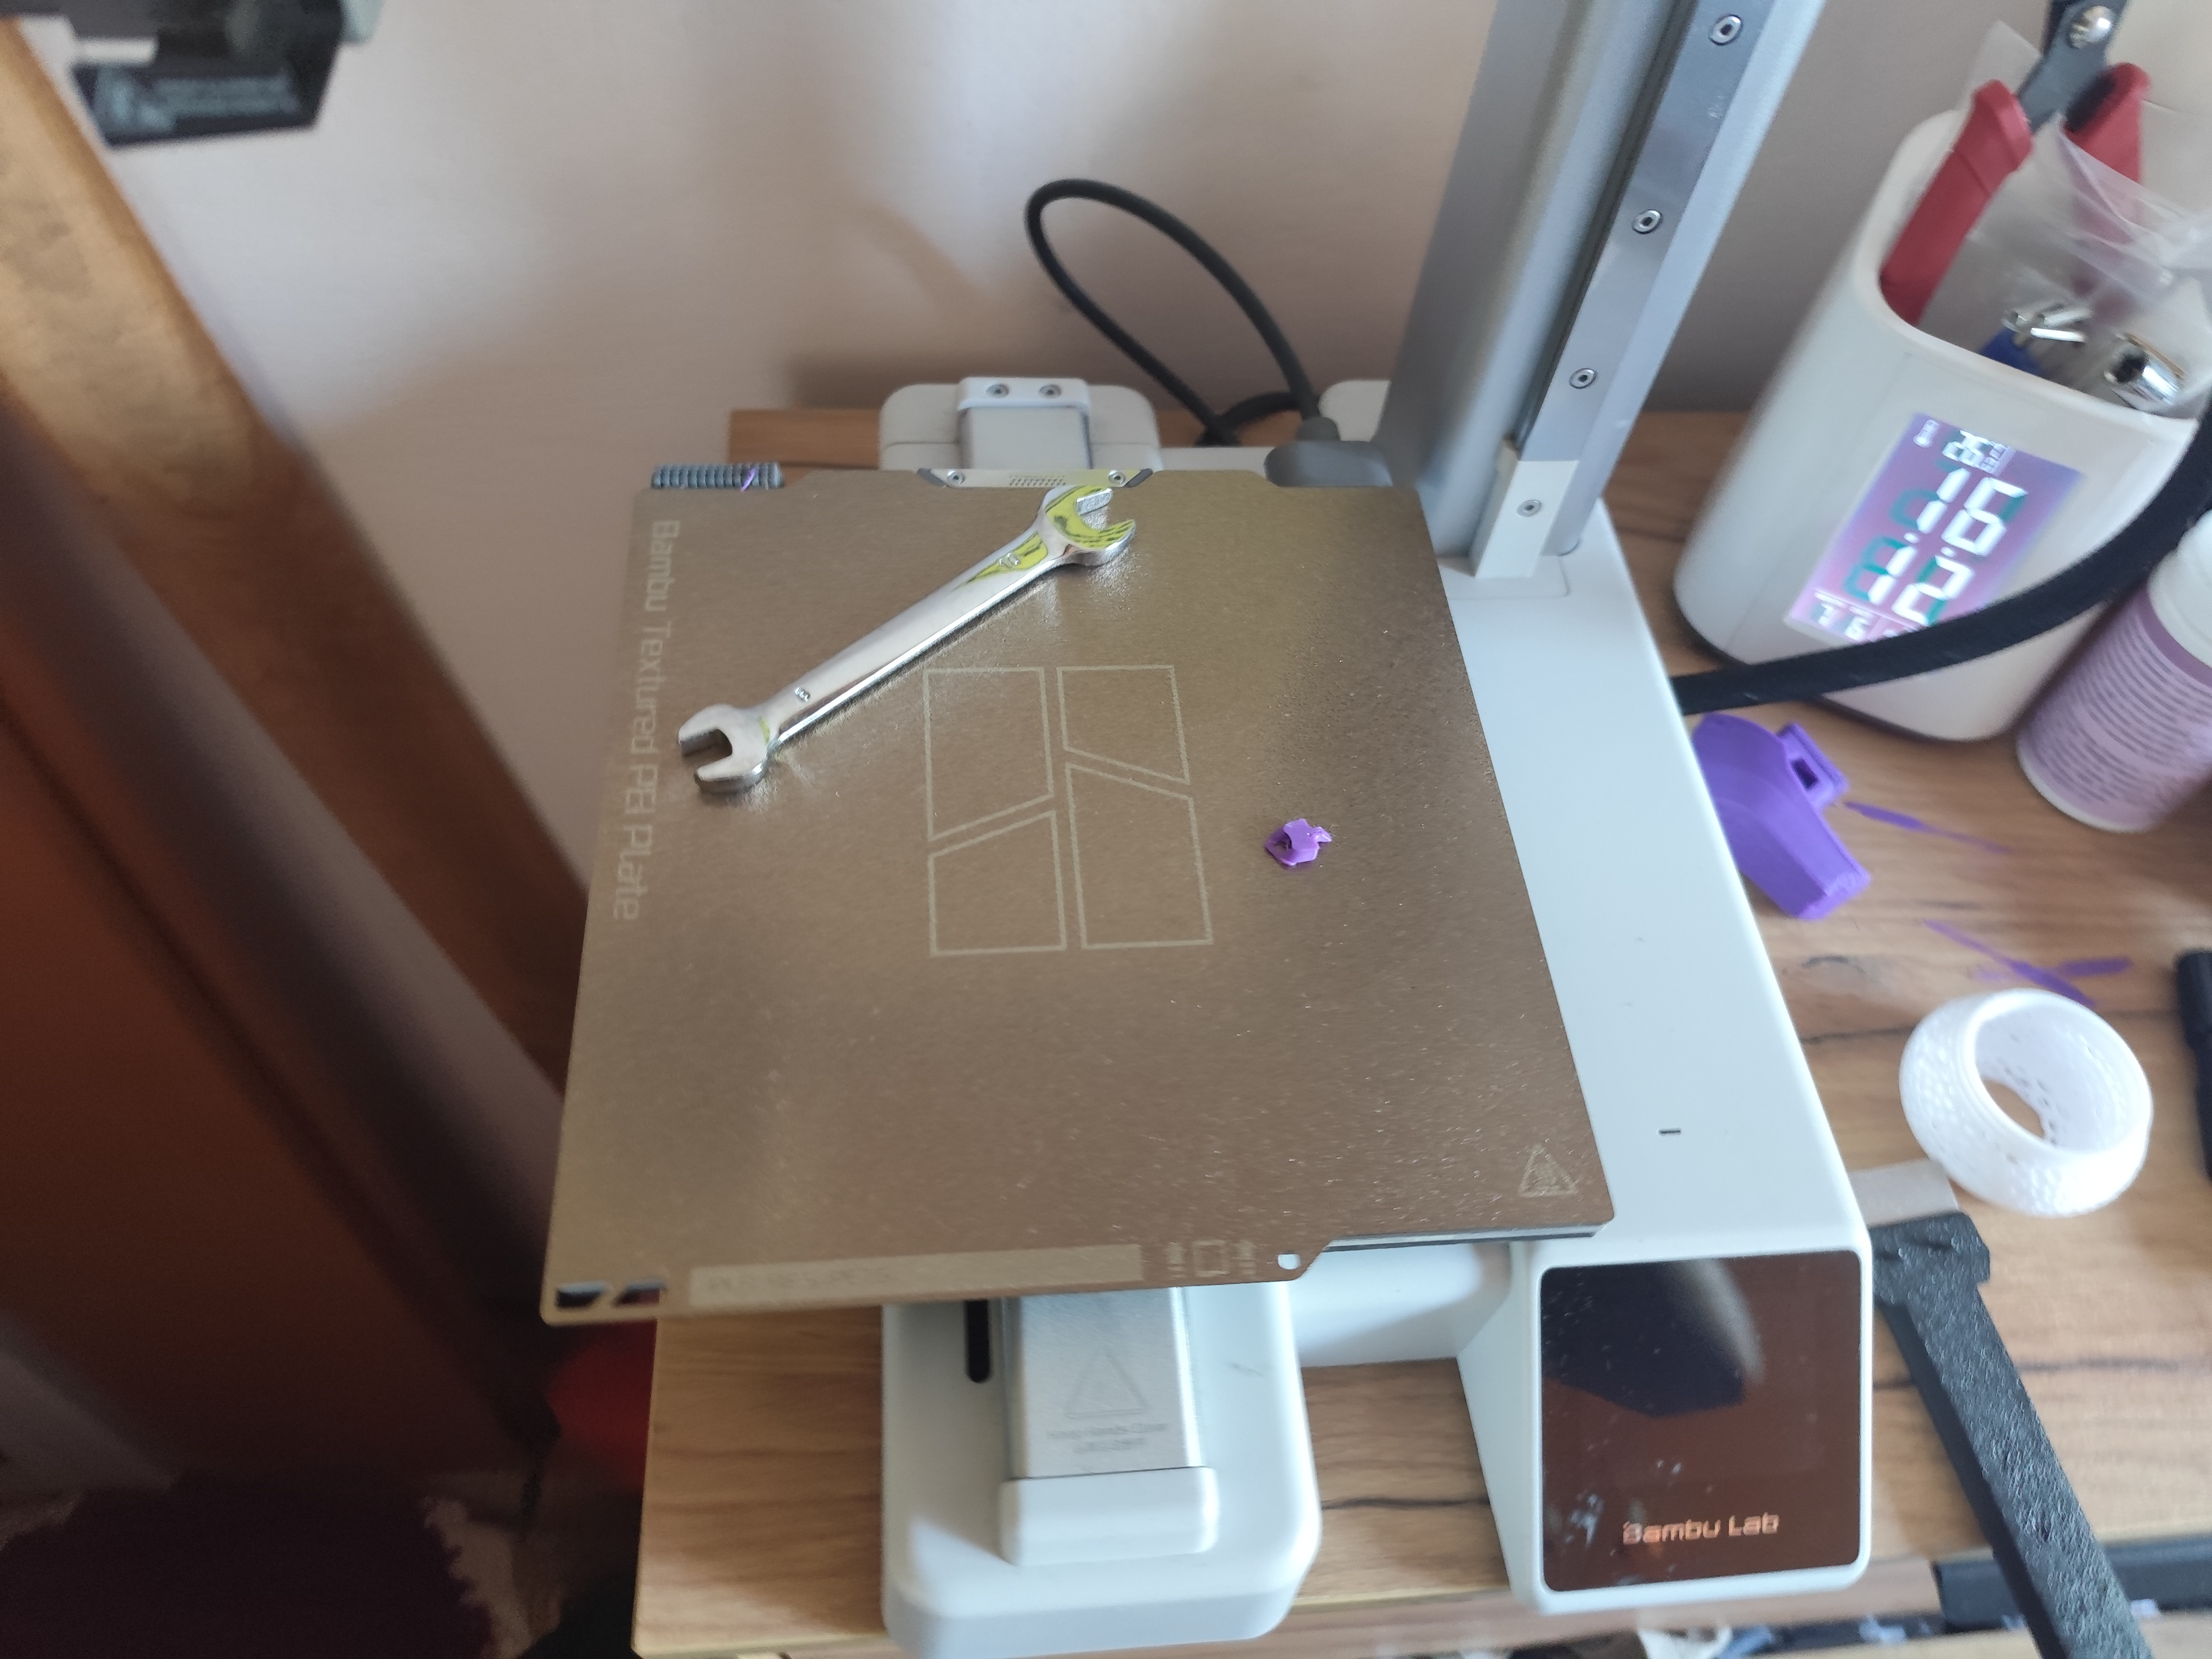
\includegraphics[width=0.3\textwidth]{figures/images/training_samples/foreign_object.jpg}
        }
        \subfigure[nem tapadó első réteg]{
            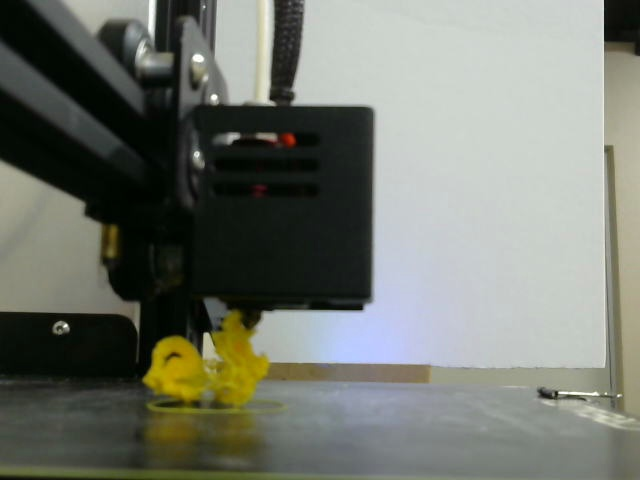
\includegraphics[width=0.3\textwidth]{figures/images/training_samples/not_sticking.jpg}
        }
        \subfigure[spagetti]{
            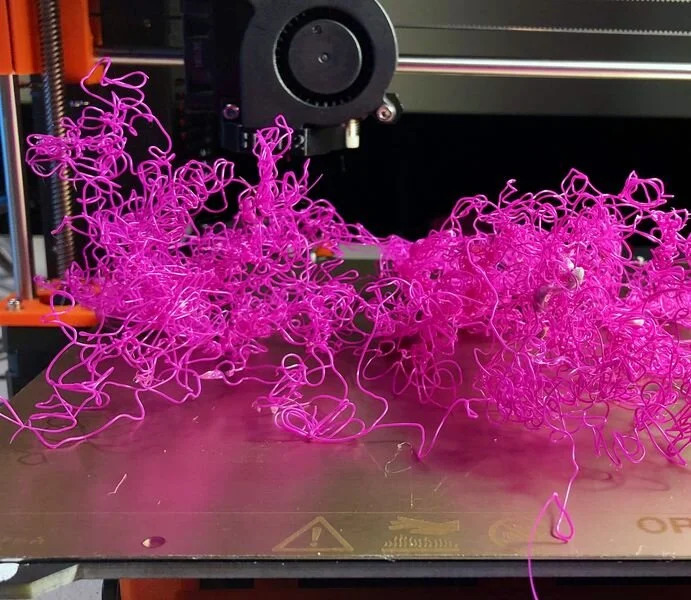
\includegraphics[width=0.3\textwidth]{figures/images/training_samples/spagetti.jpg}
        }
    \caption{Reprezentatív tanítóképek a kilenc hibaosztályból}
    \label{fig:training_grid}
    \end{figure}

    A CVAT az annotációkat YOLO-formátumban exportálta: minden képhez egy \texttt{.txt} fájl
    tartozik, amelynek minden sora egy detektált objektumot ír le az
    \texttt{<osztály> <x\_közép> <y\_közép> <szélesség> <magasság>} normalizált formátumban,
    ahol a koordináták a képmérethez viszonyítva 0 és 1 közé esnek.

    Az annotálás a projekt egyik legtöbb időt igénylő szakasza volt, mivel minden határolódobozt
    manuálisan kellett elhelyezni és az osztálycímkét hozzárendelni, különös figyelmet fordítva
    arra, hogy a több hibatípust egyidejűleg mutató képeken minden látható defektust helyesen
    azonosítsunk.

% -------------------------------------------------------------------
\section{Adathalmaz-előfeldolgozás}

    \subsection{Train/val felosztás}

    Az annotált adathalmazt a \texttt{splitter.py} szkript segítségével osztottuk szét tanító-
    és validációs részhalmazra, \textbf{80/20 arányban}. A felosztás reprodukálhatósága érdekében
    rögzített véletlenszám-magot (\texttt{seed = 42}) alkalmaztunk. Az eredményül kapott mappa-
    struktúra közvetlenül kompatibilis a YOLOv8 betanítási pipeline-jával:
    \texttt{images/train}, \texttt{images/val}, \texttt{labels/train}, \texttt{labels/val}.

    \subsection{Osztályegyensúly-korrekció - oversampling}

    Az adathalmazban a kilenc hibaosztály előfordulása nem egyenletes: egyes ritkábban előforduló
    vagy nehezebben dokumentálható hibatípusok, például a \textit{nozzle\_clog} vagy a
    \textit{foreign\_object\_on\_print\_area}, lényegesen kevesebb példánnyal szerepelnek,
    mint a gyakoribb kategóriák. Az osztályegyensúlyhiány közvetlen hatással van a modell
    tanulási dinamikájára: az alulreprezentált osztályok felismerési pontossága alacsonyabb lesz.

    Ennek korrekciójára az \texttt{oversample\_train.py} szkript osztályalapú oversamplinget
    hajt végre a tanítókészleten: minden olyan osztálynál, amelynek instanciaszáma egy meghatározott
    küszöbérték alatt marad, véletlenszerűen kiválasztott, adott osztályt tartalmazó képeket
    másol be új névvel a tanítókészletbe, legfeljebb tíz másolatot képenként, mindaddig,
    amíg a célszám el nem érhető. Ezzel az eljárással a modell az alulreprezentált hibatípusokon
    is elegendő tanulási példán tud végigmenni.

    \subsection{Adataugmentáció}

    Az adathalmaz méretének és vizuális variabilitásának növelésére automatizált augmentációs
    pipeline-t alkalmaztunk az \texttt{augment.py} szkript formájában. A szkript minden egyes
    tanítóképből alapértelmezés szerint \textbf{4 augmentált változatot} állít elő, háromféle
    augmentációs stratégia valamelyikét alkalmazva:

    \begin{itemize}
        \item \textbf{Alaptranszformációk} (~70\% valószínűséggel): Az Albumentations könyvtár
        segítségével véletlenszerű vízszintes és függőleges tükrözés, fényerő- és
        kontrasztváltoztatás, telítettség- és árnyalateltolás, Gauss-elmosás, léptékváltoztatás
        és forgatás kerül alkalmazásra, mindig a határoló dobozokat is megfelelően transzformálva.

        \item \textbf{Smart MixUp} (~20\% valószínűséggel): Két, egymással vizuálisan kompatibilis
        osztálypárt tartalmazó kép súlyozott lineáris keverékeként (\(\lambda \in [0{,}4;\,0{,}6]\))
        új szintetikus képet állít elő, amelyhez mindkét forráskép annotációi megmaradnak.
        Az összekeverhető osztálypárokat előre definiált kompatibilitási lista szabályozza,
        elkerülve a vizuálisan ellentmondásos kombinációkat.

        \item \textbf{Mozaik (\textit{Mosaic})} (~10\% valószínűséggel): Négy véletlenszerűen
        kiválasztott kép egy 640×640 pixeles vászonra kerül egymás mellé, negyed-negyed területre
        skálázva. Az így keletkező mozaikkép határoló dobozainak koordinátái átszámításra kerülnek
        az új pozícióra, megőrizve a teljes annotációt.
    \end{itemize}

    Minden augmentáció után az összes határoló doboz koordinátáit $[0, 1]$ közé visszavágjuk
    (\textit{clamping}), megelőzve az érvénytelen YOLO-annotációk keletkezését. A 4-szeres
    szorzóval végzett augmentáció eredményeként a tanítókészlet közel \textbf{négyszeresére}
    bővült, miközben a validációs halmazon augmentáció nem történt, annak érdekében, hogy
    a kiértékelés valódi, módosítatlan képeken menjen végbe.

